\chapter{Distillazione della Conoscenza in YOLO}
\label{chap:distillazione}

\section{Costruzione del Dataset Pseudo-Etichettato}
\label{sec:dist_costruzione}
Per trasferire la capacità di localizzazione dal modello teacher (DINOv3 con Linear-CAM) a un rilevatore real-time (lo studente), è stato impostato un flusso di distillazione basato su pseudo-etichettatura automatica (Figura~\ref{fig:pipeline_distillazione}).

\begin{figure}[htbp]
\centering
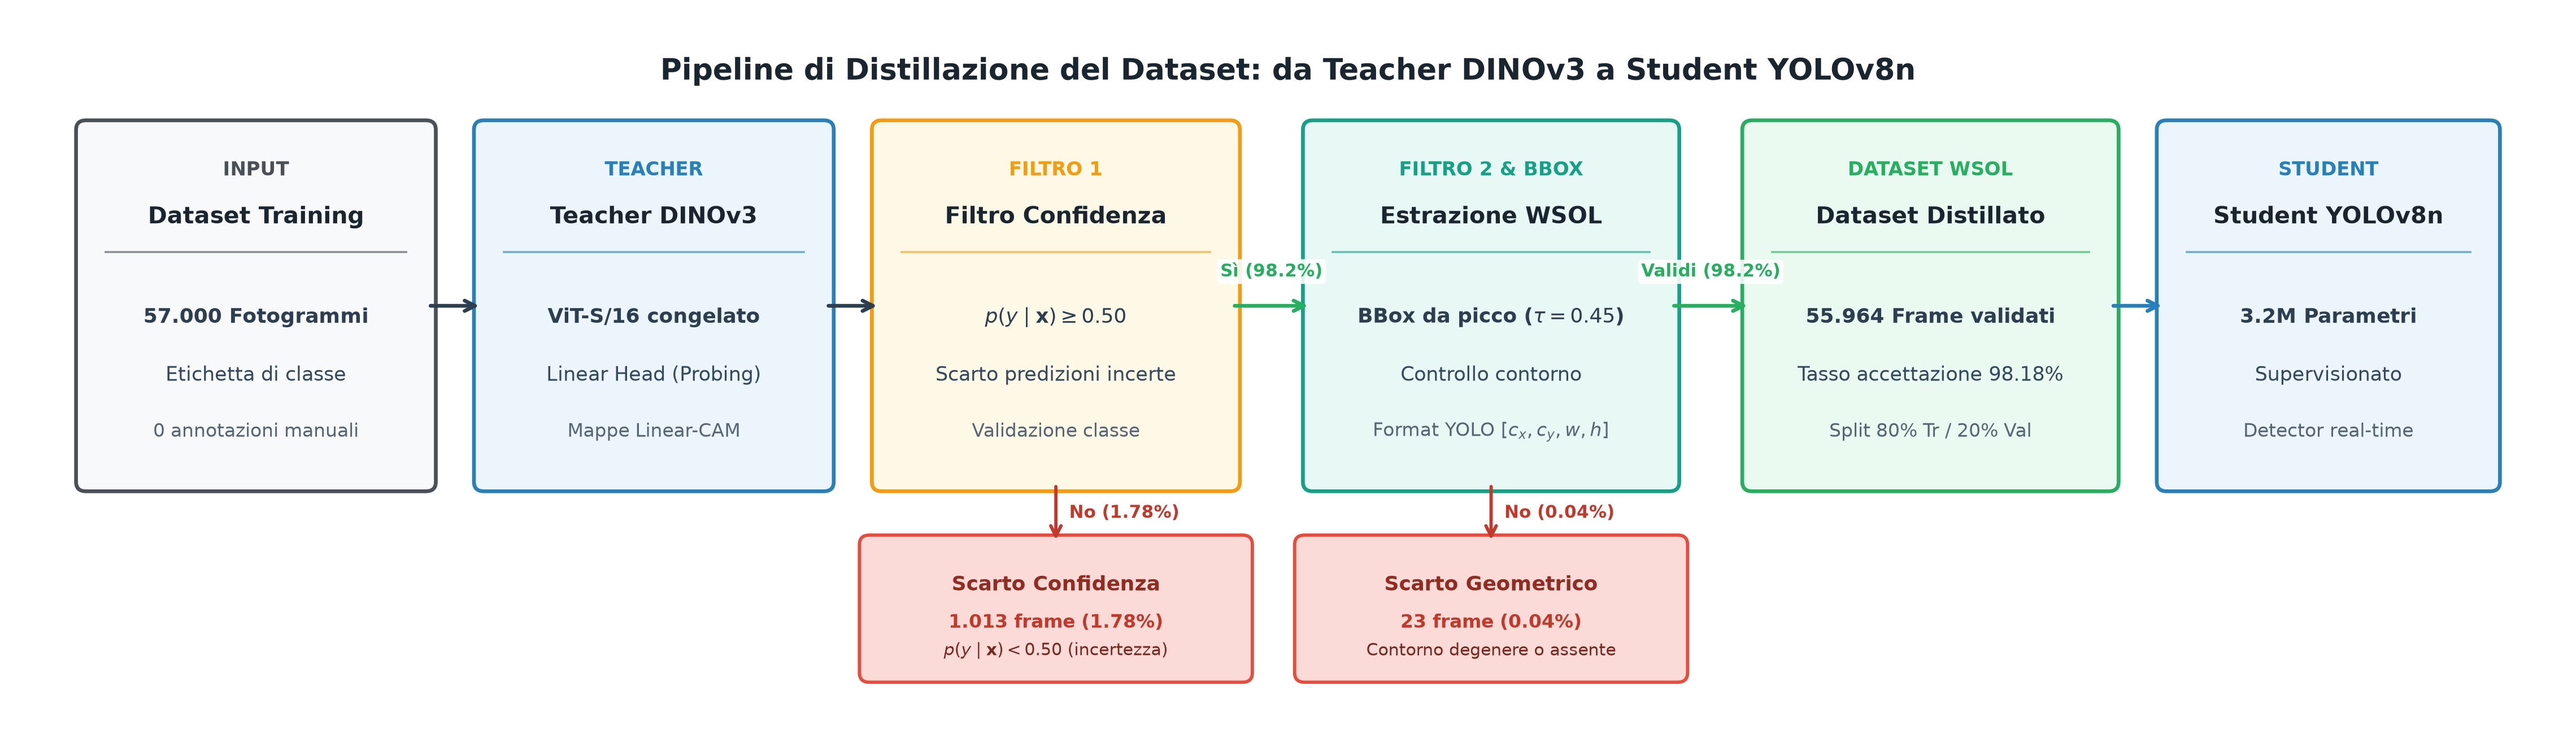
\includegraphics[width=0.95\textwidth]{figure/pipeline_distillazione.png}
\caption{Flusso di distillazione del dataset: inferenza del Teacher DINOv3, filtraggio di confidenza, estrazione dei bounding box Linear-CAM, codifica YOLO e addestramento dello Student YOLOv8n.}
\label{fig:pipeline_distillazione}
\end{figure}

\subsection{Criteri di selezione e codifica}
Per limitare il rumore nelle etichette stimate, sono stati imposti due filtri di accettazione:
\begin{enumerate}
    \item \textbf{Soglia di confidenza}: vengono tenuti solo i fotogrammi con probabilità a posteriori del classificatore $p(y \mid \mathbf{x}) \ge 0.50$.
    \item \textbf{Validità geometrica del contorno}: la mappa Linear-CAM binarizzata ($\tau = 0.45$, elemento ellittico $7 \times 7$) deve generare almeno un contorno chiuso non degenere che racchiuda il picco di attivazione.
\end{enumerate}
I vertici del rettangolo minimo $[x, y, w, h]$ sono poi normalizzati sulle dimensioni del frame $(W, H)$ secondo il formato YOLO:
$c_x = (x + w/2)/W$, $c_y = (y + h/2)/H$, $w_n = w/W$, $h_n = h/H$.

\subsection{Statistiche della distillazione}
Filtrando l'insieme di $57.000$ immagini di training con queste regole si ottengono i volumi riportati nella Tabella~\ref{tab:statistiche_distillazione}.

\begin{table}[htbp]
\centering
\small
\begin{tabularx}{\textwidth}{Lcc}
\toprule
\textbf{Categoria di Esito} & \textbf{Numero Fotogrammi} & \textbf{Percentuale} \\
\midrule
\textbf{Fotogrammi validati e pseudo-etichettati} & \textbf{55.964} & \textbf{98.18\%} \\
Scartati per confidenza insufficiente ($p < 0.50$) & $1.013$ & $1.78\%$ \\
Scartati per contorno degenere o assente & $23$ & $0.04\%$ \\
\midrule
\textbf{Totale fotogrammi elaborati} & \textbf{57.000} & \textbf{100.00\%} \\
\bottomrule
\end{tabularx}
\caption{Statistiche quantitative del processo di distillazione del dataset.}
\label{tab:statistiche_distillazione}
\end{table}

Il dataset distillato include $55.964$ fotogrammi etichettati automaticamente ($98.18\%$ del totale), senza richiedere coordinate manuali.

\section{Addestramento dello Studente (YOLOv8n)}
\label{sec:dist_student}

\subsection{Scelta architetturale}
Come modello studente è stato scelto YOLOv8n~\cite{jocher2023ultralytics} per due ragioni pratiche:
\begin{itemize}
    \item \textbf{Efficienza computazionale}: con $3.2\text{ M}$ di parametri e $8.7\text{ GFLOPs}$, supera 120 FPS su GPU standard, prestandosi all'uso su visori egocentrici o dispositivi portatili.
    \item \textbf{Capacità di regolarizzazione}: la taglia ridotta della rete limita l'overfitting sul rumore ad alta frequenza presente nei contorni estratti dalle CAM.
\end{itemize}

\subsection{Partizionamento e iperparametri}
La suddivisione tra training e validazione ricalca il criterio $80\% / 20\%$ per classe usato per DINOv3:
\begin{itemize}
    \item \textbf{Train set distillato}: $44.771$ fotogrammi;
    \item \textbf{Validation set distillato}: $11.193$ fotogrammi.
\end{itemize}
I dettagli di addestramento sono elencati nella Tabella~\ref{tab:iperparametri_yolo}.

\begin{table}[htbp]
\centering
\small
\begin{tabularx}{\textwidth}{lcL}
\toprule
\textbf{Iperparametro} & \textbf{Valore} & \textbf{Descrizione Operativa} \\
\midrule
\textbf{Risoluzione ingresso (\texttt{imgsz})} & $640 \times 640$ px & Risoluzione di default per YOLOv8 \\
\textbf{Ottimizzatore} & SGD + Momentum & Momentum $0.937$, Weight Decay $5 \times 10^{-4}$ \\
\textbf{Learning Rate iniziale (\texttt{lr0})} & $0.01$ & Decadimento lineare con warm-up iniziale \\
\textbf{Dimensione Batch} & $16$ & Con Batch Normalization \\
\textbf{Numero massimo di epoche} & $100$ & Early stopping con pazienza di 20 epoche \\
\textbf{Data Augmentation} & Mosaic, Flip, HSV & Mosaic disattivato nelle ultime 10 epoche \\
\bottomrule
\end{tabularx}
\caption{Iperparametri di addestramento di YOLOv8n sul dataset distillato.}
\label{tab:iperparametri_yolo}
\end{table}

\section{Convergenza Interna e Gap di Generalizzazione}
\label{sec:dist_gap}
Sul validation set interno (misurato rispetto alle pseudo-label del teacher), lo studente apprende a riprodurre i riquadri con alta precisione:
\begin{equation}
    \text{Val mAP@50 (Pseudo-Label)} = 96.64\%, \quad \text{Val mAP@50:95} = 86.66\%
\end{equation}
Tuttavia, valutato sul test set ufficiale ($5.462$ immagini reali verificate contro le annotazioni umane di ground truth), il modello ottiene:
\begin{equation}
    \text{Test mAP@50 (Ground Truth)} = 37.39\%, \quad \text{Test mAP@50:95} = 25.84\%
\end{equation}
Questo scarto distingue la fedeltà intra-dominio ($96.64\%$, in cui la rete impara a replicare le decisioni del teacher sullo stesso tipo di riprese) dalla generalizzazione reale sul ground truth ($37.39\%$). Sul risultato pesano il disallineamento tra le sessioni di visita e la forma intrinsecamente approssimata dei contorni generati dalle CAM rispetto ai box umani. Il capitolo successivo inserisce questo risultato nel protocollo comparativo di sample efficiency.
